% Options for packages loaded elsewhere
\PassOptionsToPackage{unicode}{hyperref}
\PassOptionsToPackage{hyphens}{url}
%
\documentclass[
]{article}
\usepackage{amsmath,amssymb}
\usepackage{lmodern}
\usepackage{iftex}
\ifPDFTeX
  \usepackage[T1]{fontenc}
  \usepackage[utf8]{inputenc}
  \usepackage{textcomp} % provide euro and other symbols
\else % if luatex or xetex
  \usepackage{unicode-math}
  \defaultfontfeatures{Scale=MatchLowercase}
  \defaultfontfeatures[\rmfamily]{Ligatures=TeX,Scale=1}
\fi
% Use upquote if available, for straight quotes in verbatim environments
\IfFileExists{upquote.sty}{\usepackage{upquote}}{}
\IfFileExists{microtype.sty}{% use microtype if available
  \usepackage[]{microtype}
  \UseMicrotypeSet[protrusion]{basicmath} % disable protrusion for tt fonts
}{}
\makeatletter
\@ifundefined{KOMAClassName}{% if non-KOMA class
  \IfFileExists{parskip.sty}{%
    \usepackage{parskip}
  }{% else
    \setlength{\parindent}{0pt}
    \setlength{\parskip}{6pt plus 2pt minus 1pt}}
}{% if KOMA class
  \KOMAoptions{parskip=half}}
\makeatother
\usepackage{xcolor}
\IfFileExists{xurl.sty}{\usepackage{xurl}}{} % add URL line breaks if available
\IfFileExists{bookmark.sty}{\usepackage{bookmark}}{\usepackage{hyperref}}
\hypersetup{
  hidelinks,
  pdfcreator={LaTeX via pandoc}}
\urlstyle{same} % disable monospaced font for URLs
\usepackage[margin=1in]{geometry}
\usepackage{longtable,booktabs,array}
\usepackage{calc} % for calculating minipage widths
% Correct order of tables after \paragraph or \subparagraph
\usepackage{etoolbox}
\makeatletter
\patchcmd\longtable{\par}{\if@noskipsec\mbox{}\fi\par}{}{}
\makeatother
% Allow footnotes in longtable head/foot
\IfFileExists{footnotehyper.sty}{\usepackage{footnotehyper}}{\usepackage{footnote}}
\makesavenoteenv{longtable}
\usepackage{graphicx}
\makeatletter
\def\maxwidth{\ifdim\Gin@nat@width>\linewidth\linewidth\else\Gin@nat@width\fi}
\def\maxheight{\ifdim\Gin@nat@height>\textheight\textheight\else\Gin@nat@height\fi}
\makeatother
% Scale images if necessary, so that they will not overflow the page
% margins by default, and it is still possible to overwrite the defaults
% using explicit options in \includegraphics[width, height, ...]{}
\setkeys{Gin}{width=\maxwidth,height=\maxheight,keepaspectratio}
% Set default figure placement to htbp
\makeatletter
\def\fps@figure{htbp}
\makeatother
\setlength{\emergencystretch}{3em} % prevent overfull lines
\providecommand{\tightlist}{%
  \setlength{\itemsep}{0pt}\setlength{\parskip}{0pt}}
\setcounter{secnumdepth}{5}
\usepackage{booktabs}
\usepackage{longtable}
\usepackage{array}
\usepackage{multirow}
\usepackage{wrapfig}
\usepackage{float}
\usepackage{colortbl}
\usepackage{pdflscape}
\usepackage{tabu}
\usepackage{threeparttable}
\usepackage{threeparttablex}
\usepackage[normalem]{ulem}
\usepackage{makecell}
\usepackage{xcolor}
\ifLuaTeX
  \usepackage{selnolig}  % disable illegal ligatures
\fi

\author{}
\date{\vspace{-2.5em}}

\begin{document}

\hypertarget{data-analysis}{%
\section{Data Analysis}\label{data-analysis}}

To compare latent process correlation between those who transitioned to MCI or dementia during follow-up and those who did not, we fit the MLLT model which allows correlation in the observation errors and underlying cognitive process (OS) using the model of interest described in section \ref{MOI}. The model is fit on the full data and sensitivity analysis matched data described in section \ref{DAT}. The Gibb's sampling was repeated 5,000 times with a burn-in of 2,000 samples, resulting in 3,000 samples for parameter interest. Non-informative priors are used for both the linear effects and covariance matrices.

\hypertarget{data-analysis-results}{%
\subsection{Data Analysis Results}\label{data-analysis-results}}

In both the dementia and non-dementia groups, there is very little estimated observation correlation. Instead, the correlation is primarily placed in the state equation. For the state correlation, in the non-dementia population there are much distinct correlation clusters in memory (LOGIMEM, MEMUNITS), digit (DIGIB, DIGIF), and executive function (TRAILA, TRAILB, WAIS). The dementia population generally has much higher correlation in the state equation. The digit and executive function blocks share much higher cross correlation than the non-dementia group. The Animals test generally has low correlation for the non-dementia population and very high correlation with all tests the other tests in the population that transitioned to MCI or dementia.

As expected by the correlation estimates, 23 of the 36 correlation coefficients share less than 5\% overlap in posterior draw distributions.

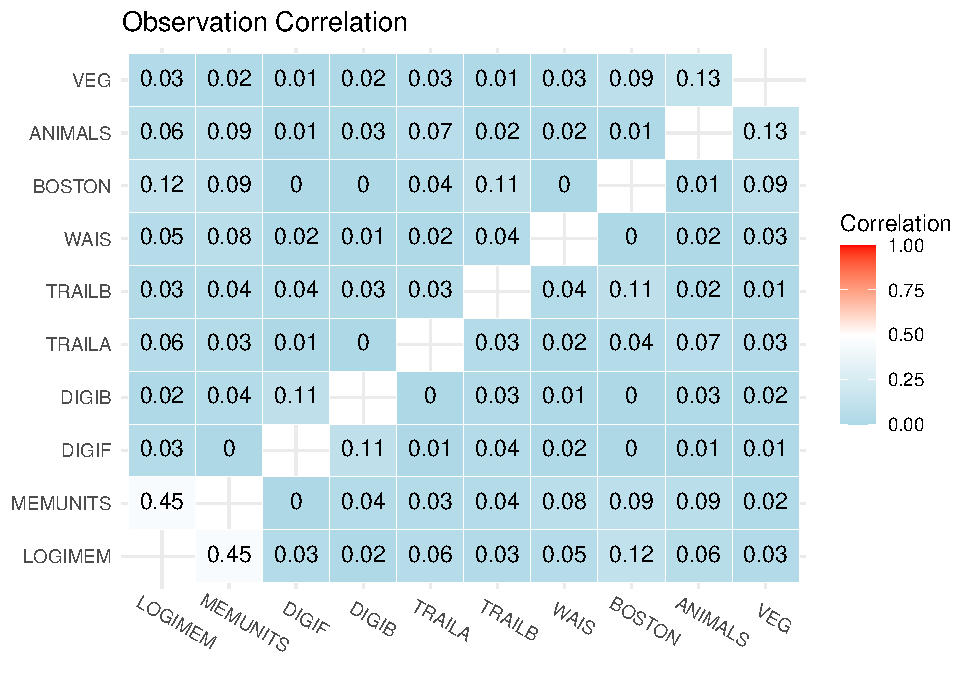
\includegraphics{DataAnalysis_files/figure-latex/unnamed-chunk-3-1.pdf}

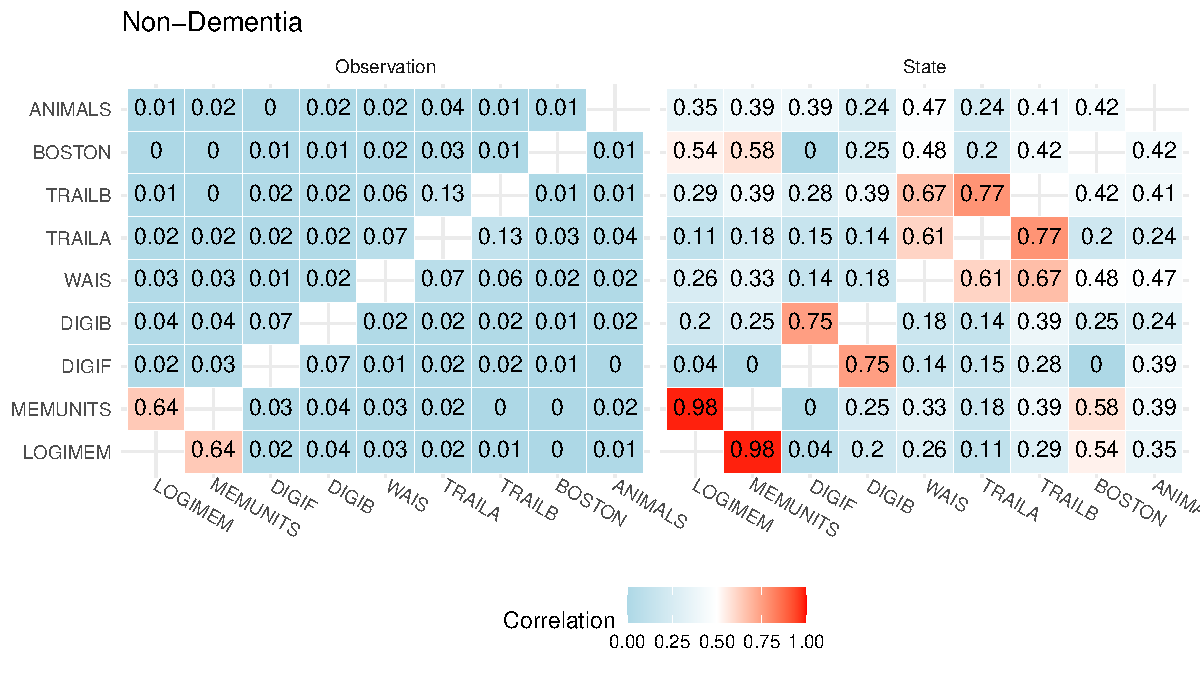
\includegraphics{DataAnalysis_files/figure-latex/unnamed-chunk-5-1.pdf}

\hypertarget{state-correlation-posterior-differences}{%
\subsubsection{State Correlation Posterior Differences}\label{state-correlation-posterior-differences}}

h

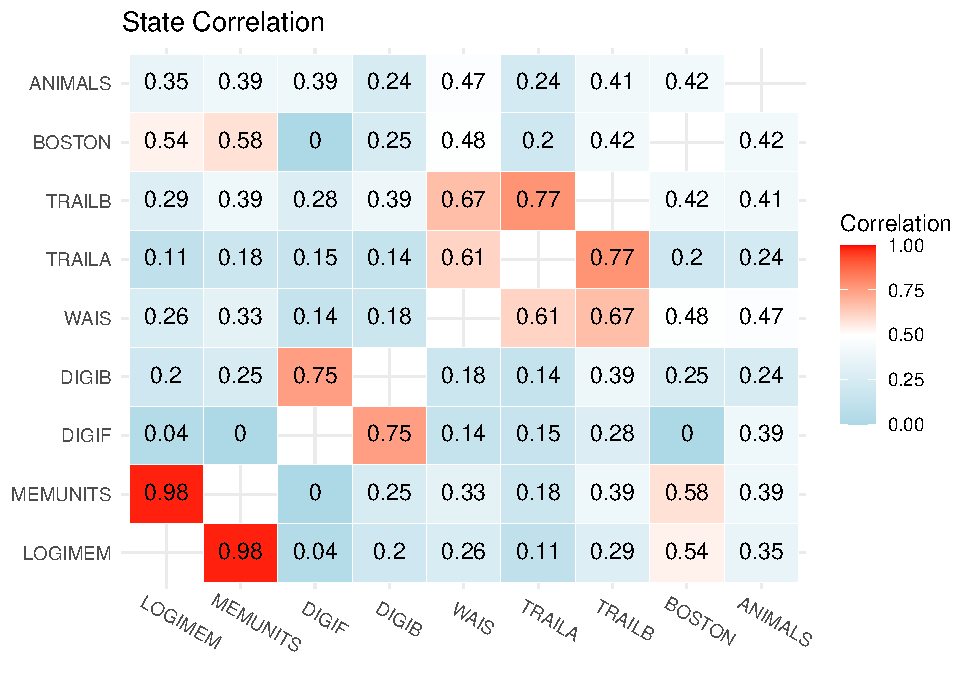
\includegraphics{DataAnalysis_files/figure-latex/unnamed-chunk-7-1.pdf}

\begin{itemize}
\tightlist
\item
  \textbf{BLUE} is \textbf{Non-Dementia}
\item
  \textbf{RED} is \textbf{Dementia}
\end{itemize}

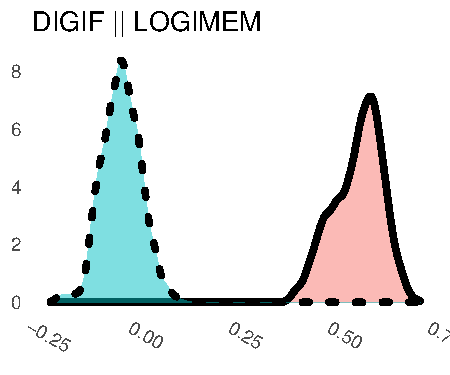
\includegraphics{DataAnalysis_files/figure-latex/unnamed-chunk-8-1.pdf} 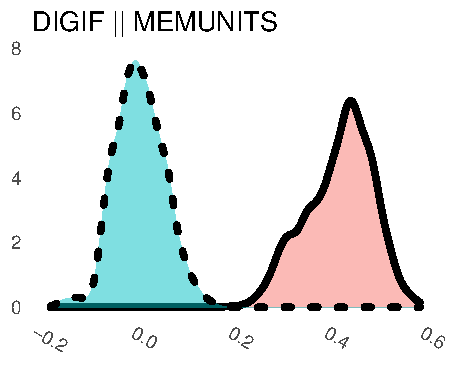
\includegraphics{DataAnalysis_files/figure-latex/unnamed-chunk-8-2.pdf} 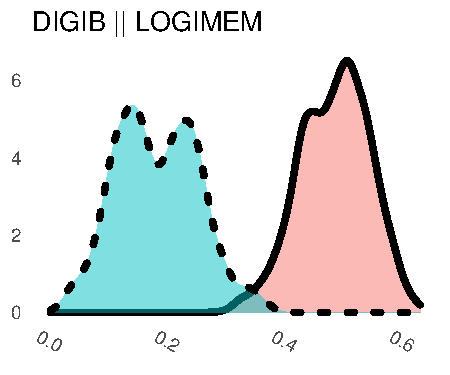
\includegraphics{DataAnalysis_files/figure-latex/unnamed-chunk-8-3.pdf} 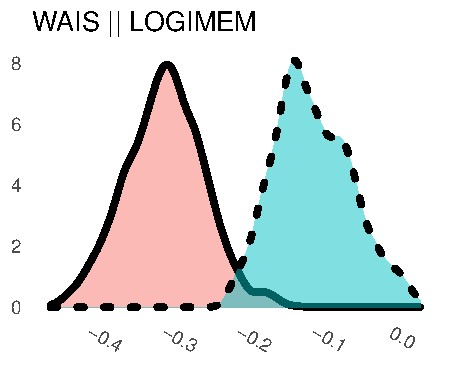
\includegraphics{DataAnalysis_files/figure-latex/unnamed-chunk-8-4.pdf} 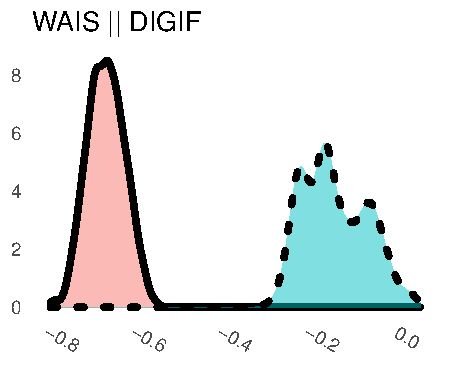
\includegraphics{DataAnalysis_files/figure-latex/unnamed-chunk-8-5.pdf} 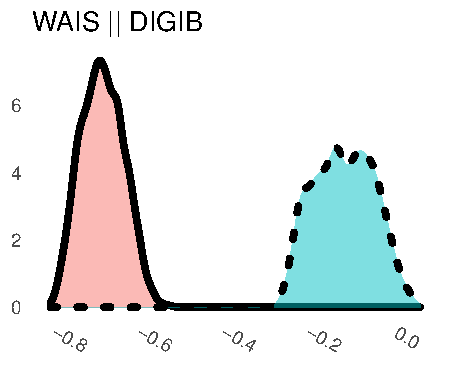
\includegraphics{DataAnalysis_files/figure-latex/unnamed-chunk-8-6.pdf} 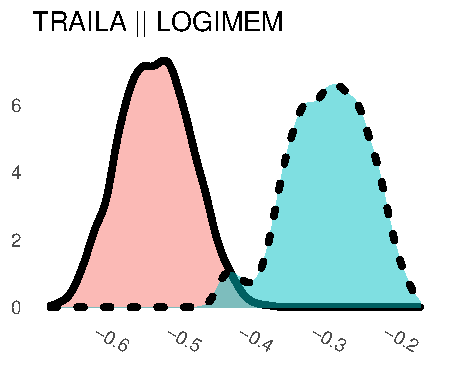
\includegraphics{DataAnalysis_files/figure-latex/unnamed-chunk-8-7.pdf} 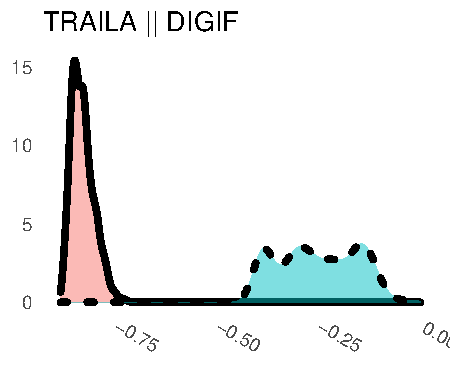
\includegraphics{DataAnalysis_files/figure-latex/unnamed-chunk-8-8.pdf} 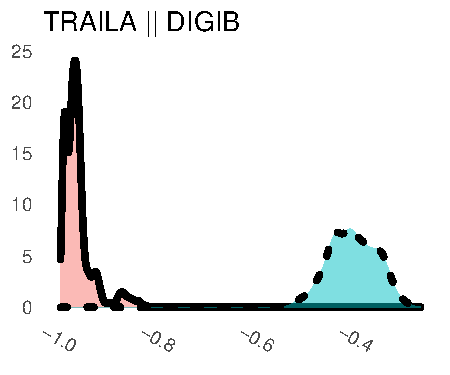
\includegraphics{DataAnalysis_files/figure-latex/unnamed-chunk-8-9.pdf} 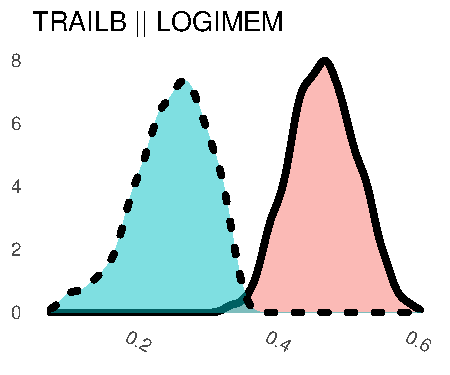
\includegraphics{DataAnalysis_files/figure-latex/unnamed-chunk-8-10.pdf} 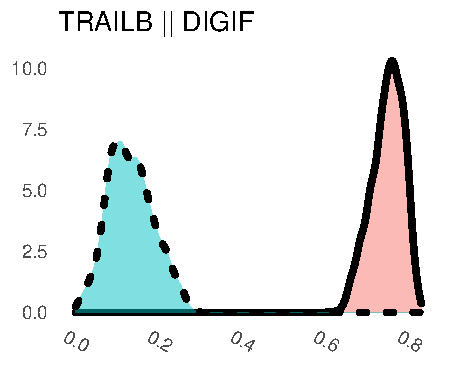
\includegraphics{DataAnalysis_files/figure-latex/unnamed-chunk-8-11.pdf} 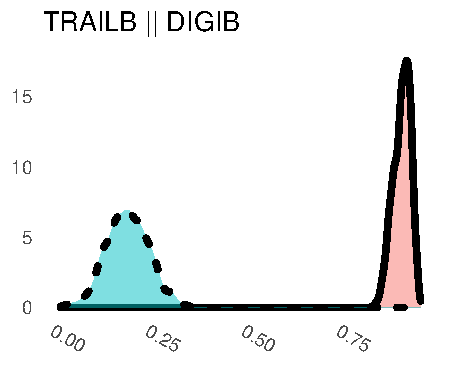
\includegraphics{DataAnalysis_files/figure-latex/unnamed-chunk-8-12.pdf} 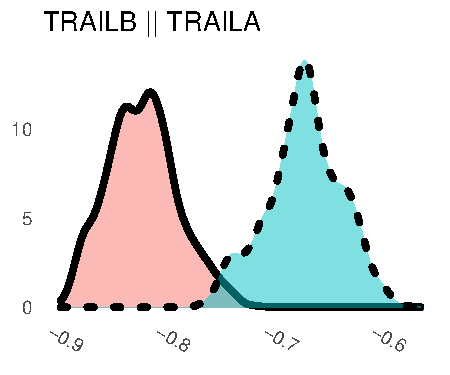
\includegraphics{DataAnalysis_files/figure-latex/unnamed-chunk-8-13.pdf} 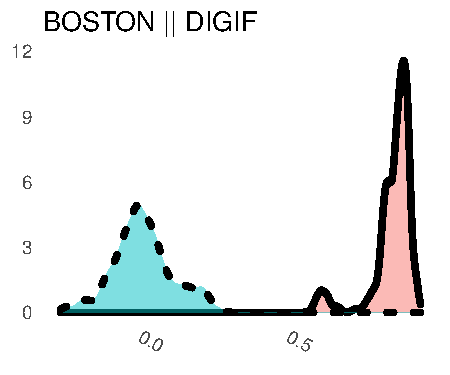
\includegraphics{DataAnalysis_files/figure-latex/unnamed-chunk-8-14.pdf} 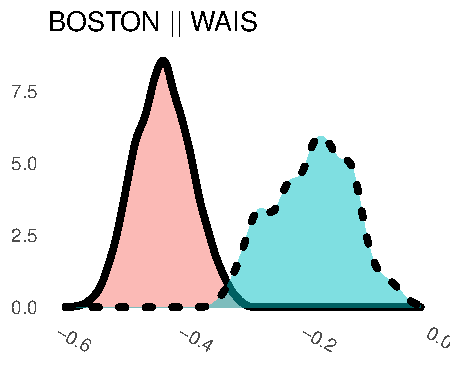
\includegraphics{DataAnalysis_files/figure-latex/unnamed-chunk-8-15.pdf} 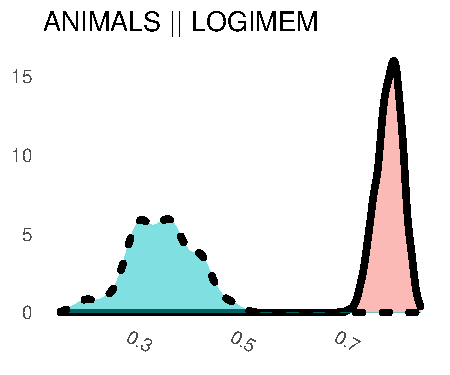
\includegraphics{DataAnalysis_files/figure-latex/unnamed-chunk-8-16.pdf} 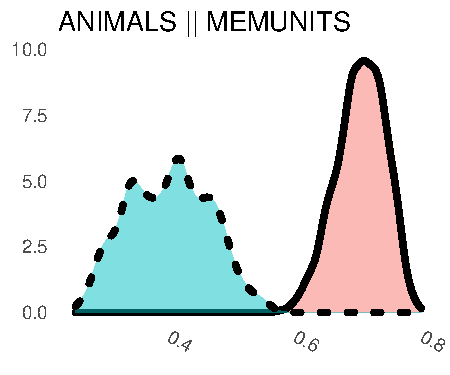
\includegraphics{DataAnalysis_files/figure-latex/unnamed-chunk-8-17.pdf} 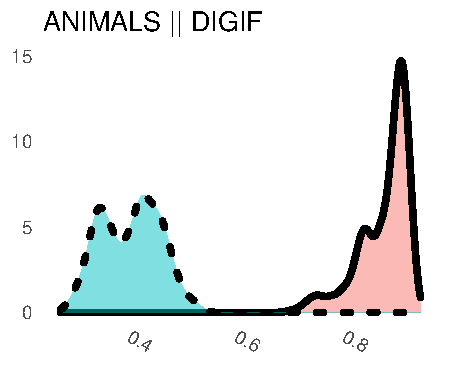
\includegraphics{DataAnalysis_files/figure-latex/unnamed-chunk-8-18.pdf} 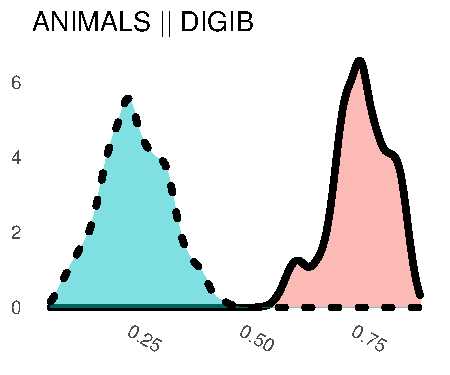
\includegraphics{DataAnalysis_files/figure-latex/unnamed-chunk-8-19.pdf} 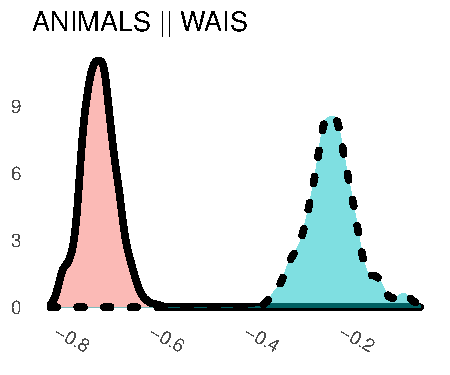
\includegraphics{DataAnalysis_files/figure-latex/unnamed-chunk-8-20.pdf} 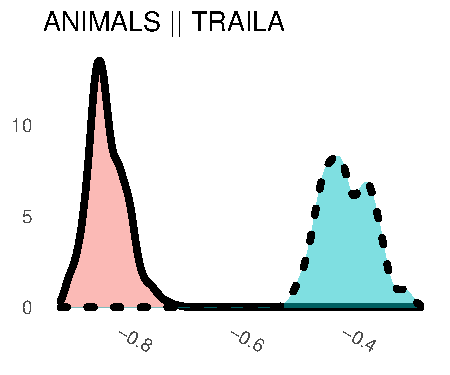
\includegraphics{DataAnalysis_files/figure-latex/unnamed-chunk-8-21.pdf} 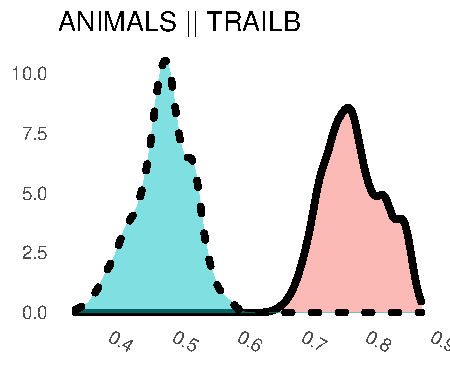
\includegraphics{DataAnalysis_files/figure-latex/unnamed-chunk-8-22.pdf} 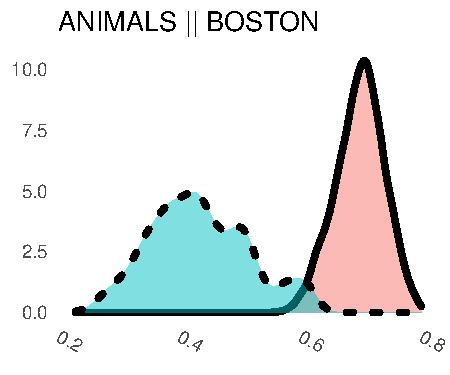
\includegraphics{DataAnalysis_files/figure-latex/unnamed-chunk-8-23.pdf}

\hypertarget{sensitivity}{%
\subsubsection{Sensitivity}\label{sensitivity}}

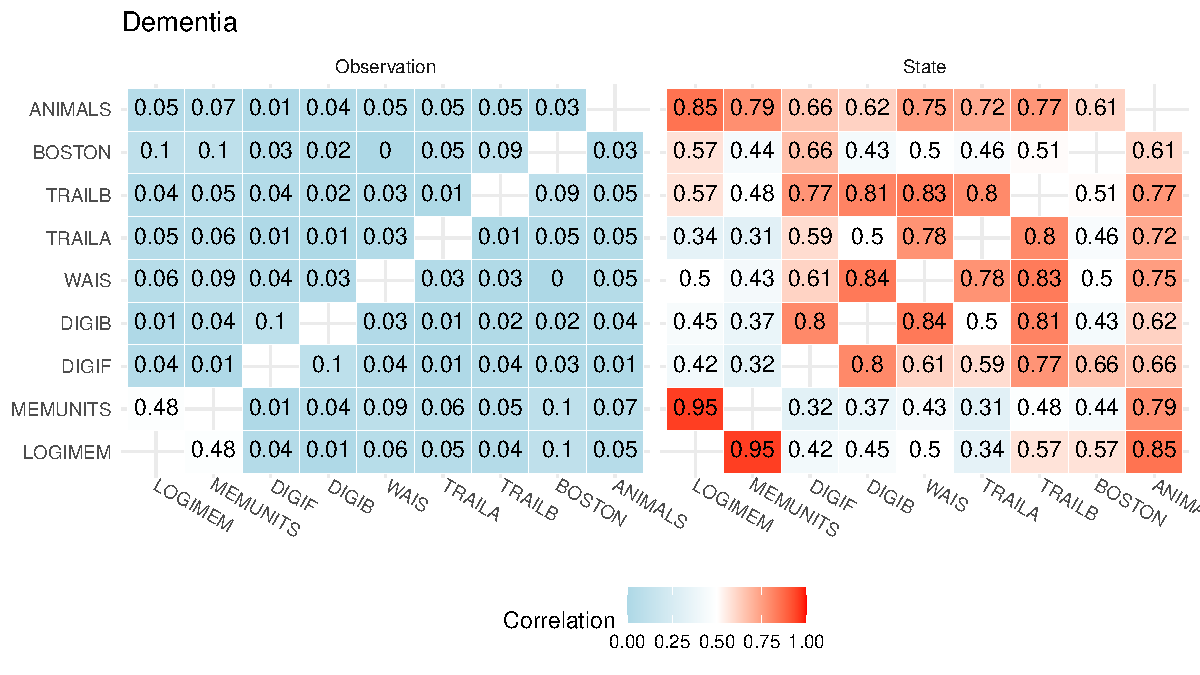
\includegraphics{DataAnalysis_files/figure-latex/unnamed-chunk-9-1.pdf}

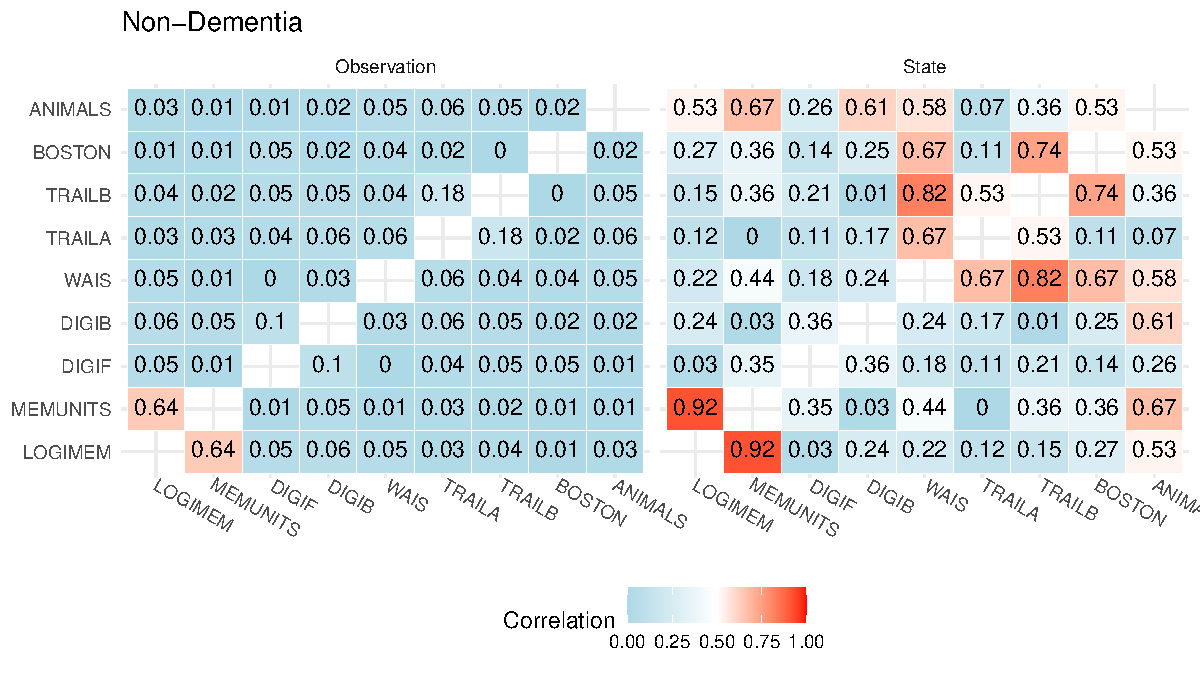
\includegraphics{DataAnalysis_files/figure-latex/unnamed-chunk-10-1.pdf}

\end{document}
